\section{Algorithm Overview}\label{sec:algorithm}

In analyzing the performance of methods from the previous section, we make two observations:

\begin{enumerate}
\item Global computations (such as a global scan) are expensive, and approaches to multisplit that require many rounds, each with a global computation, are likely to be uncompetitive. Any reduction in the cost of global computation is desirable.
\item After we derive the permutation, the cost of permuting the elements with a global scatter (consecutive input elements going into arbitrarily distant final destinations) is also expensive.
This is primarily because of the non-coalesced memory accesses associated with the scatter. Any increase in memory locality associated with the scatter is also desirable.
\end{enumerate}

The key design insight in this paper is that we can reduce the cost of both global computation and global scatter at the cost of doing more local work, and that doing so is beneficial for overall performance. We begin by describing and analyzing a framework for the different approaches we study in this paper, then discuss the generic structure common to all our implementations.

\subsection{Our parallel model}\label{subsec:parallel_model}
Multisplit cannot be solved by using only local operations; i.e., we cannot divide a multisplit problem into two independent subparts and solve each part locally without any communication between the two parts. We thus assume any viable implementation must include at least a single global operation to gather necessary global information from all elements (or group of elements).
We generalize the approaches we study in this paper into a series of $N$ rounds, where each round has 3 stages: a set of local operations (which run in parallel on independent subparts of the global problem); a global operation (across all subparts); and another set of local operations. In short: \textbraceleft local, global, local\textbraceright, repeated $N$ times; in this paper we refer to these three stages as \textbraceleft prescan, scan, postscan\textbraceright.

The approaches from Section~\ref{sec:init_approaches} all fit this model. Scan-based split starts by making a flag vector (where the local level is per-thread), performing a global scan operation on all flags, and then ordering the results into their final positions (thread-level local). The iterative (or recursive) scan-based split with $m$ buckets repeats the above approach for $m$ (or $\lceil \log m \rceil$) rounds.
Radix sort also requires several rounds. Each round starts by identifying a bit (or a group of bits) from its keys (local), running a global scan operation, and then locally moving data such that all keys are now sorted based on the selected bit (or group of bits).
In radix sort literature, these stages are mostly known as up-sweep, scan and down-sweep.
Reduced-bit sort is derived from radix sort; the main differences are that in the first round, the label vector and the new packed values are generated locally (thread-level), and in the final round, the packed key-value pairs are locally unpacked (thread-level) to form the final results.

\subsection{Multisplit requires a global computation}
Let's explore the global and local components of stable multisplit, which together compute a unique permutation of key-value pairs into their final positions.
Suppose we have $m$ buckets $B_0, B_1, \dots, B_{m-1}$, each with $h_0, h_1, \dots, h_{m-1}$ elements respectively ($\sum_i{h_i} = n$, where $n$ is the total number of elements).
If $u_i \in B_j$ is the $i$th element in key vector $\mathbf{u}$, then its final permuted position $p(i)$ should be (from $u_i$'s perspective):
\begin{equation}\label{eq:permutation}
        p(i) = \underbrace{\sum_{k = 0}^{j-1}h_k}_{\text{global offset}} + \underbrace{\left| \{u_r \in B_j: r < i\}\right|}_{\text{local offset ($u_i$'s bucket)}},
\end{equation}
where $|\cdot|$ is the cardinality operator that denotes the number of elements within its set argument. The left term is the total number of key elements that belong to the preceding buckets, and the right term is the total number of preceding elements (with respect to $u_i$) in $u_i$'s bucket, $B_j$.
Computing both of these terms in this form and for all elements (for all $i$) requires global operations (e.g., computing a histogram of buckets).

\subsection{Dividing multisplit into subproblems}\label{subsec:2levels}
Equation~\eqref{eq:permutation} clearly shows what we need in order to compute each permutation (i.e., final destinations for a stable multisplit solution): a histogram of buckets among all elements ($h_k$) as well as local offsets for all elements within the same bucket (the second term). However, it lacks intuition about how we should compute each term.
Both terms in equation~\eqref{eq:permutation}, at their core, answer the following question: to which bucket does each key belong? If we answer this question for every key and for all buckets (hypothetically, for each bucket we store a binary bitmap variable of length $n$ to show all elements that belong to that bucket), then each term can be computed intuitively as follows: 1)~histograms are equal to counting all elements in each bucket (reduction of a specific bitmap); 2)~local offsets are equivalent to counting all elements from the beginning to that specific index and within the same bucket (scan operation on a specific bitmap).
This intuition is closely related to our definition of the scan-based split method in Section~\ref{sec:scan_split}. However, it is practically not competitive because it requires storing huge bitmaps (total of $mn$ binary variables) and then performing global operations on them.

Although the above solution seems impractical for a large number of keys, it seems more favorable for input problems that are small enough.
As an extreme example, suppose we wish to perform multisplit on a single key. Each bitmap variable becomes just a single binary bit. Performing reduction and scan operations become as trivial as whether a single bit is set or not.
Thus, a divide-and-conquer approach seems like an appealing solution to solve equation~\eqref{eq:permutation}: we would like to divide our main problem into small enough subproblems such that solving each subproblem is ``easy'' for us. By an easy computation we mean that it is either small enough so that we can afford to process it sequentially, or that instead we can use an efficient parallel hardware alternative (such as the GPU's ballot instruction). When we solve a problem directly in this way, we call it a \emph{direct solve}.
Next, we formalize our divide-and-conquer formulation.

Let us divide our input key vector $\mathbf{u}$ into $L$ contiguous subproblems: $\mathbf{u} = [\mathbf{u}_{0}, \mathbf{u}_{1}, \dots, \mathbf{u}_{L-1}]$. Suppose each subvector $\mathbf{u}_\ell$ has $h_{0,\ell}, h_{1,\ell}, \dots, h_{m-1,\ell}$ elements in buckets $B_0, B_1, \dots B_{m-1}$ respectively.
For example, for arbitrary values of $i$, $s$, and $j$ such that key item $u_i \in \mathbf{u}_s$ and $u_i$ is in bucket $B_j$, equation~\eqref{eq:permutation} can be rewritten as (from $u_i$'s perspective):
\begin{equation}\label{eq:permutation2}
p(i) = \underbrace{\overbrace{\sum_{k=0}^{j-1}\left(\sum_{\ell = 0}^{L-1}h_{k,\ell}\right)}^{\text{previous buckets}}+\overbrace{\sum_{\ell=0}^{s-1}h_{j,\ell}}^\text{$u_i$'s bucket}}_\text{global offset}
 + \underbrace{\left| \{u_r \in \mathbf{u}_s: (u_r \in B_j) \land (r < i)\}\right|}_{\text{local offset within $u_i$'s subproblem}}.
 \end{equation}
This formulation has two separate parts. The first and second terms require global computation (first: the element count of all preceding buckets across all subproblems, and second: the element count of the same bucket in all preceding subproblems). The third term can be computed locally within each subproblem. Note that equation~\eqref{eq:permutation} and~\eqref{eq:permutation2}'s first terms are equivalent (total number of previous buckets), but the second term in~\eqref{eq:permutation} is broken into the second and third terms in~\eqref{eq:permutation2}.

The first and second terms can both be computed with a global histogram computed over $L$ local histograms. A global histogram is generally implemented with global scan operations (here, exclusive prefix-sum). We can characterize this histogram as a scan over a 2-dimensional matrix  $\mathbf{H} = [h_{i,\ell}]_{m\times L}$, where the ``height'' of the matrix is the bucket count $m$ and the ``width'' of the matrix is the number of subproblems $L$\@.
The second term can be computed by a scan operation of size $L$ on each row (total of $m$ scans for all buckets). The first term will be a single scan operation of size $m$ over the reduction of all rows (first reduce each row horizontally to compute global histograms and then scan the results vertically). Equivalently, both terms can be computed by a single scan operation of size $mL$ over a row-vectorized $\mathbf{H}$.
Either way, the cost of our global operation is roughly proportional to both $m$ and $L$\@. We see no realistic way to reduce $m$. Thus we concentrate on reducing $L$\@.

\subsection{Hierarchical approach toward multisplit localization}\label{subsec:localization}
We prefer to have small enough subproblems ($\bar{n}$) so that our local computations are ``easy'' for a direct solve. For any given subproblem size, we will have $L = n/\bar{n}$ subproblems to be processed globally as described before.
On the other hand, we want to minimize our global computations as well, because they require synchronization among all subproblems and involve (expensive) global memory accesses.
So, with a fixed input size and a fixed number of buckets ($n$ and $m$), we would like to both decrease our subproblem size and number of subproblems, which is indeed paradoxical.

Our solution is a hierarchical approach. We do an arbitrary number of levels of divide-and-conquer, until at the last level, subproblems are small enough to be solved easily and directly (our preferred $\bar{n}$).
These results are then appropriately combined together to eventually reach the first level of the hierarchy, where now we have a reasonable number of subproblems to be combined together using global computations (our preferred $L$).

Another advantage of such an approach is that, in case our hardware provides a memory hierarchy with smaller but faster local memory storage (as GPUs do with register level and shared memory level hierarchies, as opposed to the global memory), we can potentially perform all computations related to all levels except the first one in our local memory hierarchies without any global memory interaction.
Ideally, we would want to use all our available register and shared memory with our subproblems to solve them locally, and then combine the results using global operations.
In practice, however, since our local memory storage options are very limited, such solution may still lead to a large number of subproblems to be combined with global operations (large $L$).
As a result, by adding more levels of hierarchy (than the available memory hierarchies in our device) we can systematically organize the way we fill our local memories, process them locally, store intermediate results, and then proceed to the next batch, which overall reduces our global operations.
 Next, we will theoretically consider such a hierarchical approach (\emph{multi-level localization}) and explore the changes to equation~\eqref{eq:permutation2}.

\begin{figure}
  \centering
  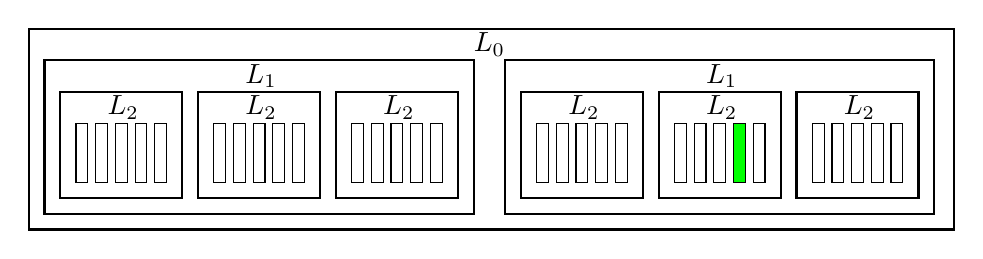
\begin{tikzpicture}[every node/.style={thick,rectangle,inner sep=0pt}]
\def \dx {0.1}
\def \dy {0.2}
\def \recx {0.15}
\def \recX {5*\recx + 6*\dx}
\def \recXX {3 * \recX + 26 * \dx}
\def \recy {0.75}
\def \recY {\recy + 3 * \dy}
\def \recYY {\recY + 3 * \dy}

%% left child 
\draw [black] (0 + 0, 0 + 0) rectangle (0 + \recx, 0 + \recy);
\draw [black] (0 + \recx + \dx, 0) rectangle (0 + 2*\recx + \dx, 0 + \recy);
\draw [black] (0 + 2*\recx + 2*\dx, 0 + 0) rectangle (0 + 3*\recx + 2*\dx, 0 + \recy);
\draw [black] (0 + 3*\recx + 3*\dx, 0 + 0) rectangle (0 + 4*\recx + 3*\dx, 0 + \recy);
\draw [black] (0 + 4*\recx + 4*\dx, 0 + 0) rectangle (0 + 5*\recx + 4*\dx, 0 + \recy);

\draw[thick, black] (0-2*\dx, 0-\dy) rectangle (0-2*\dx + \recX + 2 * \dx, 0-\dy + \recY);
\node () at (0 + 2 * \recx + 3 * \dx, \recy + \dy) {$L_2$};

\draw [black] (\recX + 4*\dx + 0, 0 + 0) rectangle (\recX + 4*\dx + \recx, 0 + \recy);
\draw [black] (\recX + 4*\dx + \recx + \dx, 0) rectangle (\recX + 4*\dx + 2*\recx + \dx, 0 + \recy);
\draw [black] (\recX + 4*\dx + 2*\recx + 2*\dx, 0 + 0) rectangle (\recX + 4*\dx + 3*\recx + 2*\dx, 0 + \recy);
\draw [black] (\recX + 4*\dx + 3*\recx + 3*\dx, 0 + 0) rectangle (\recX + 4*\dx + 4*\recx + 3*\dx, 0 + \recy);
\draw [black] (\recX + 4*\dx + 4*\recx + 4*\dx, 0 + 0) rectangle (\recX + 4*\dx + 5*\recx + 4*\dx, 0 + \recy);

\draw[thick, black] (\recX + 4*\dx-2*\dx, 0-\dy) rectangle (\recX + 4*\dx-2*\dx + \recX + 2 * \dx, 0-\dy + \recY);
\node () at (\recX + 4*\dx + 2 * \recx + 3 * \dx, \recy + \dy) {$L_2$};

\draw [black] (2*\recX + 14*\dx + 0, 0 + 0) rectangle (2*\recX + 14*\dx + \recx, 0 + \recy);
\draw [black] (2*\recX + 14*\dx + \recx + \dx, 0) rectangle (2*\recX + 14*\dx + 2*\recx + \dx, 0 + \recy);
\draw [black] (2*\recX + 14*\dx + 2*\recx + 2*\dx, 0 + 0) rectangle (2*\recX + 14*\dx + 3*\recx + 2*\dx, 0 + \recy);
\draw [black] (2*\recX + 14*\dx + 3*\recx + 3*\dx, 0 + 0) rectangle (2*\recX + 14*\dx + 4*\recx + 3*\dx, 0 + \recy);
\draw [black] (2*\recX + 14*\dx + 4*\recx + 4*\dx, 0 + 0) rectangle (2*\recX + 14*\dx + 5*\recx + 4*\dx, 0 + \recy);

\draw[thick, black] (2*\recX + 14*\dx-2*\dx, 0-\dy) rectangle (2*\recX + 14*\dx-2*\dx + \recX + 2 * \dx, 0-\dy + \recY);
\node () at (2*\recX + 14*\dx + 2 * \recx + 3 * \dx, \recy + \dy) {$L_2$};

\draw [thick, black] (0-4*\dx, 0-2*\dy) rectangle (0-4*\dx + \recXX, 0-2*\dy + \recYY);
\node () at (\recX + 4*\dx + 2 * \recx + 3 * \dx, \recy + 3* \dy) {$L_1$};

%% second tile
\draw [black] (\recXX + 4*\dx + 0, 0 + 0) rectangle (\recXX + 4 * \dx + \recx, 0 + \recy);
\draw [black] (\recXX + 4*\dx + \recx + \dx, 0) rectangle (\recXX + 4 * \dx + 2*\recx + \dx, 0 + \recy);
\draw [black] (\recXX + 4*\dx + 2*\recx + 2*\dx, 0 + 0) rectangle (\recXX + 4 * \dx + 3*\recx + 2*\dx, 0 + \recy);
\draw [black] (\recXX + 4*\dx + 3*\recx + 3*\dx, 0 + 0) rectangle (\recXX + 4 * \dx + 4*\recx + 3*\dx, 0 + \recy);
\draw [black] (\recXX + 4*\dx + 4*\recx + 4*\dx, 0 + 0) rectangle (\recXX + 4 * \dx + 5*\recx + 4*\dx, 0 + \recy);

\draw[thick, black] (\recXX + 4*\dx-2*\dx, 0-\dy) rectangle (\recXX + 4 * \dx-2*\dx + \recX + 2 * \dx, 0-\dy + \recY);
\node () at (\recXX + 4*\dx + 3*\dx + 2 * \recx, \recy + \dy) {$L_2$};

\draw [black] (\recXX + 4*\dx + \recX + 4*\dx + 0, 0 + 0) rectangle (\recXX + 4*\dx + \recX + 4*\dx + \recx, 0 + \recy);
\draw [black] (\recXX + 4*\dx + \recX + 4*\dx + \recx + \dx, 0) rectangle (\recXX + 4*\dx + \recX + 4*\dx + 2*\recx + \dx, 0 + \recy);
\draw [black] (\recXX + 4*\dx + \recX + 4*\dx + 2*\recx + 2*\dx, 0 + 0) rectangle (\recXX + 4*\dx + \recX + 4*\dx + 3*\recx + 2*\dx, 0 + \recy);
\fill [green] (\recXX + 4*\dx + \recX + 4*\dx + 3*\recx + 3*\dx, 0 + 0) rectangle (\recXX + 4*\dx + \recX + 4*\dx + 4*\recx + 3*\dx, 0 + \recy);
\draw [black] (\recXX + 4*\dx + \recX + 4*\dx + 3*\recx + 3*\dx, 0 + 0) rectangle (\recXX + 4*\dx + \recX + 4*\dx + 4*\recx + 3*\dx, 0 + \recy);
\draw [black] (\recXX + 4*\dx + \recX + 4*\dx + 4*\recx + 4*\dx, 0 + 0) rectangle (\recXX + 4*\dx + \recX + 4*\dx + 5*\recx + 4*\dx, 0 + \recy);

\draw[thick, black] (\recXX + 4*\dx + \recX + 4*\dx-2*\dx, 0-\dy) rectangle (\recXX + 4*\dx + \recX + 4*\dx-2*\dx + \recX + 2 * \dx, 0-\dy + \recY);
\node () at (\recXX + 4*\dx + \recX + 4*\dx + 2 * \recx + 3 * \dx, \recy + \dy) {$L_2$};

\draw [black] (\recXX + 4*\dx + 2*\recX + 14*\dx + 0, 0 + 0) rectangle (\recXX + 4*\dx + 2*\recX + 14*\dx + \recx, 0 + \recy);
\draw [black] (\recXX + 4*\dx + 2*\recX + 14*\dx + \recx + \dx, 0) rectangle (\recXX + 4*\dx + 2*\recX + 14*\dx + 2*\recx + \dx, 0 + \recy);
\draw [black] (\recXX + 4*\dx + 2*\recX + 14*\dx + 2*\recx + 2*\dx, 0 + 0) rectangle (\recXX + 4*\dx + 2*\recX + 14*\dx + 3*\recx + 2*\dx, 0 + \recy);
\draw [black] (\recXX + 4*\dx + 2*\recX + 14*\dx + 3*\recx + 3*\dx, 0 + 0) rectangle (\recXX + 4*\dx + 2*\recX + 14*\dx + 4*\recx + 3*\dx, 0 + \recy);
\draw [black] (\recXX + 4*\dx + 2*\recX + 14*\dx + 4*\recx + 4*\dx, 0 + 0) rectangle (\recXX + 4*\dx + 2*\recX + 14*\dx + 5*\recx + 4*\dx, 0 + \recy);

\draw[thick, black] (\recXX + 4*\dx + 2*\recX + 14*\dx-2*\dx, 0-\dy) rectangle (\recXX + 4*\dx + 2*\recX + 14*\dx-2*\dx + \recX + 2 * \dx, 0-\dy + \recY);
\node () at (\recXX + 4*\dx + 2*\recX + 14*\dx + 2 * \recx + 3 * \dx, \recy + \dy) {$L_2$};

\draw [thick, black] (\recXX + 4*\dx + 0-4*\dx, 0-2*\dy) rectangle (\recXX + 4*\dx + 0-4*\dx + \recXX, 0-2*\dy + \recYY);
\node () at (\recXX + 4*\dx + \recX + 4*\dx + 2 * \recx + 3 * \dx, \recy + 3* \dy) {$L_1$};

%% outer rectangle:
\draw [thick, black] (0-6*\dx, 0 - 3 * \dy) rectangle (0-6*\dx + 3*\recXX + 12*\dx + 6*\dx, 0-3*\dy + \recYY + 3*\dy);
\node () at (\recXX -2* \dx, \recYY -\dy) {$L_0$};

% \def\dx{1}
% \def\a{0}
% \def\recx{0.15}
% \def\recy{0.75}
% \node (a1) at (0 * \dx,0) [draw, minimum width=\recx cm, minimum height=\recy cm, anchor=north] {};
% \node (ap1) at (0.25 * \dx,0) [draw, minimum width=\recx cm, minimum height=\recy cm, anchor=north] {};
% \node (ap1) at (0.5 * \dx,0) [draw, minimum width=\recx cm, minimum height=\recy cm, anchor=north] {};
% \node (ap1) at (0.75 * \dx,0) [draw, minimum width=\recx cm, minimum height=\recy cm, anchor=north] {};
% \node (a2) at (1*\dx,0) [draw, minimum width=\recx cm, minimum height=\recy cm, anchor=north] {};

% \node (a3) at (2*\dx,0) [draw, minimum width=\recx cm, minimum height=\recy cm, anchor=north] {};
% \node (ap3) at (2.25*\dx,0) [draw, minimum width=\recx cm, minimum height=\recy cm, anchor=north] {};
% \node (ap3) at (2.5*\dx,0) [draw, minimum width=\recx cm, minimum height=\recy cm, anchor=north] {};
% \node (ap3) at (2.75*\dx,0) [draw, minimum width=\recx cm, minimum height=\recy cm, anchor=north] {};
% \node (a4) at (3*\dx,0) [draw, minimum width=\recx cm, minimum height=\recy cm, anchor=north] {};

% \node (a5) at (4*\dx,0) [draw, minimum width=\recx cm, minimum height=\recy cm, anchor=north] {};
% \node (ap5) at (4.25*\dx,0) [draw, minimum width=\recx cm, minimum height=\recy cm, anchor=north] {};
% \node (ap5) at (4.5*\dx,0) [draw, minimum width=\recx cm, minimum height=\recy cm, anchor=north] {};
% \node (ap5) at (4.75*\dx,0) [draw, minimum width=\recx cm, minimum height=\recy cm, anchor=north] {};
% \node (a6) at (5*\dx,0) [draw, minimum width=\recx cm, minimum height=\recy cm, anchor=north] {};

% \node (a7) at (6*\dx + \a,0) [draw, minimum width=\recx cm, minimum height=\recy cm, anchor=north] {};
% \node (ap7) at (6.25*\dx + \a,0) [draw, minimum width=\recx cm, minimum height=\recy cm, anchor=north] {};
% \node (ap7) at (6.5*\dx + \a,0) [draw, minimum width=\recx cm, minimum height=\recy cm, anchor=north] {};
% \node (ap7) at (6.75*\dx + \a,0) [draw, minimum width=\recx cm, minimum height=\recy cm, anchor=north] {};
% \node (a8) at (7*\dx+ \a,0) [draw, minimum width=\recx cm, minimum height=\recy cm, anchor=north] {};

% \node (a9) at (8*\dx+ \a,0) [draw, minimum width=\recx cm, minimum height=\recy cm, anchor=north] {};
% \node (ap9) at (8.25*\dx+ \a,0) [draw, minimum width=\recx cm, minimum height=\recy cm, anchor=north] {};
% \node (ap9) at (8.5*\dx+ \a,0) [draw, minimum width=\recx cm, minimum height=\recy cm, anchor=north] {};
% \node (app9) at (8.75*\dx+ \a,0) [draw, minimum width=\recx cm, minimum height=\recy cm, anchor=north, fill=green] {};
% \node (a10) at (9*\dx+ \a,0) [draw, minimum width=\recx cm, minimum height=\recy cm, anchor=north] {};

% \draw[->] (app9) -- (8.75*\dx + \a, -1.65);
% \node (text) at (8.75*\dx + \a + 0.1, -1.75) {\scriptsize$(1,1,3)$};

% \node (a11) at (10*\dx+ \a,0) [draw, minimum width=\recx cm, minimum height=\recy cm, anchor=north] {};
% \node (ap11) at (10.25*\dx+ \a,0) [draw, minimum width=\recx cm, minimum height=\recy cm, anchor=north] {};
% \node (ap11) at (10.5*\dx+ \a,0) [draw, minimum width=\recx cm, minimum height=\recy cm, anchor=north] {};
% \node (ap11) at (10.75*\dx+ \a,0) [draw, minimum width=\recx cm, minimum height=\recy cm, anchor=north] {};
% \node (a12) at (11*\dx+ \a,0) [draw, minimum width=\recx cm, minimum height=\recy cm, anchor=north] {};

% \node (b1) [draw, minimum width=10*\recx cm, minimum height=2*\recy cm, anchor=north, label=$L_2$, fit = (a1)(a2), rounded corners=0.1cm] {};
% \node (b2) [draw, minimum width=10*\recx cm, minimum height=2*\recy cm, anchor=north, label=$L_2$, fit = (a3)(a4), rounded corners=0.1cm] {};
% \node (b3) [draw, minimum width=10*\recx cm, minimum height=2*\recy cm, anchor=north, label=$L_2$, fit = (a5)(a6), rounded corners=0.1cm] {};

% \node (b4) [draw, minimum width=10*\recx cm, minimum height=2*\recy cm, anchor=north, label=$L_2$, fit = (a7)(a8), rounded corners=0.1cm] {};
% \node (b5) [draw, minimum width=10*\recx cm, minimum height=2*\recy cm, anchor=north, label=$L_2$, fit = (a9)(a10), rounded corners=0.1cm] {};
% \node (b6) [draw, minimum width=10*\recx cm, minimum height=2*\recy cm, anchor=north, label=$L_2$, fit = (a11)(a12), rounded corners=0.1cm] {};

% \node (c1) [draw, minimum width=38*\recx cm, minimum height=3* \recy cm, anchor=north, label=$L_1$, fit = (b1)(b2)(b3), rounded corners=0.1cm] {};
% \node (c2) [draw, minimum width=38*\recx cm, minimum height=3* \recy cm, anchor=north, label=$L_1$, fit = (b4)(b5)(b6), rounded corners=0.1cm] {};

% \node (d1) [draw, minimum width=80*\recx cm, minimum height=4 * \recy cm, anchor=north, label=$L_0$, fit = (c1)(c2), rounded corners=0.1cm] {};

\end{tikzpicture}
  \caption{An example for our localization terminology. Here we have 3 levels of localization with $L_0 = 2$, $L_1 = 3$ and $L_2 = 5$. For example, the marked subproblem (in green) can be addressed by a tuple $(1,1,3)$ where each index respectively denotes its position in the hierarchical structure.\label{fig:localization}}
\end{figure}

% Consider a hierarchical approach, such that we continue our divisions: we divide each subproblem into several smaller subsubproblems, and continue to do so.
\paragraph{$\lambda$-level localization}
For any given set of arbitrary non-zero integers $\{L_0, L_1, \dots, L_{\lambda - 1}\}$, we can perform $\lambda$ levels of localizations as follows: Suppose we initially divide our problem into $L_0$ smaller parts. These divisions form our first level (i.e., the \emph{global level}).
Next, each subproblem at the first level is divided into $L_1$ smaller subproblems to form the second level. We continue this process until the $\lambda$th level (with $L_{\lambda-1}$ subproblems each). Figure~\ref{fig:localization} shows an example of our hierarchical division of the multisplit problem.
There are total of $L_\text{total} = L_0 \times L_1 \times \dots L_{\lambda - 1}$ smaller problems and their results should be hierarchically added together to compute the final permutation $p(i)$.
Let $(\ell_0,\ell_1,\dots,\ell_{\lambda-1})$ denote a subproblem's position in our hierarchical tree: $\ell_0$th branch from the first level, $\ell_1$th branch from the second level, and so forth until the last level.
Among all elements within this subproblem, we count those that belong to bucket $B_i$ as $h_{i,(\ell_0,\dots,\ell_{\lambda-1})}$.
Similar to our previous permutation computation, for an arbitrary $i$, $j$, and $(s_0,\dots,s_{\lambda-1})$, suppose $u_i \in \mathbf{u}_{(s_0, \dots, s_{\lambda-1})}$ and $u_i \in B_j$.
We can write $p(i)$ as follows (from $u_i$'s perspective):

\begin{IEEEeqnarray}{rCl}\label{eq:permutation3}
p(i) & = & \sum_{k = 0}^{j-1}\left(\sum_{\ell_0 = 0}^{L_0 - 1} \sum_{\ell_1 = 0}^{L_1 - 1} \dots \sum_{\ell_{\lambda - 1} = 0}^{L_{\lambda - 1} - 1}h_{k, (\ell_0, \ell_1, \dots, \ell_{\lambda-1})}\right)
\hfill \rightarrow \text{\scriptsize previous buckets in the whole problem} \nonumber \\
&& +\: \sum_{\ell_0 = 0}^{s_0 - 1}\left(\sum_{\ell_1 = 0}^{L_1-1}\dots\sum_{\ell_{\lambda-1}=0}^{L_{\lambda-1} - 1}{h_{j,(\ell_0,\ell_1,\dots,\ell_{\lambda-1})}}\right)
\hfill\rightarrow \text{\scriptsize $u_i$'s bucket, first level, previous subproblems} \nonumber \\
&& +\: \sum_{\ell_1 = 0}^{s_1 - 1}\left(\sum_{\ell_2 = 0}^{L_2-1}\dots\sum_{\ell_{\lambda-1}=0}^{L_{\lambda-1} - 1}{h_{j,(s_0,\ell_1,\ell_2,\dots,\ell_{\lambda-1})}}\right)
\hfill\rightarrow \text{\scriptsize $u_i$'s bucket, second level, previous subproblems} \nonumber \\
&& \vdots \hfill\rightarrow \text{\scriptsize $u_i$'s bucket, previous levels, previous subproblems} \nonumber \\
&& +\: \sum_{\ell_{\lambda-1} = 0}^{s_{\lambda-1} - 1}h_{j,(s_0,\dots,s_{\lambda-2},\ell_{\lambda-1})}
\hfill\rightarrow \text{\scriptsize $u_i$'s bucket, last level, previous subproblems} \nonumber \\
&& +\: \left| \left\{u_r \in \mathbf{u}_{(s_0, \dots, s_{\lambda-1})}: (u_r \in B_j) \land (r < i)\right\}\right|.
\hfill\rightarrow \text{\scriptsize $u_i$'s bucket, $u_i$'s subproblem} \nonumber \\
\end{IEEEeqnarray}

There is an important resemblance between this equation and equation~\eqref{eq:permutation2}. The first and second terms (from top to bottom) are similar, with the only difference that each $h_{k,\ell}$ is now further broken into $L_1\times \dots \times L_{\lambda-1}$ subproblems (previously it was just $L = L_0$ subproblems). The other terms of \eqref{eq:permutation3} can be seen as a hierarchical disintegration of the local offset in \eqref{eq:permutation2}.

Similar to Section~\ref{subsec:2levels}, we can form a matrix $\mathbf{H} = [h_{j,\ell_0}]_{m\times L_0}$ for global computations where
\begin{equation}
h_{j,\ell_0} = \sum_{\ell_1 = 0}^{L_1-1}\dots\sum_{\ell_{\lambda-1} = 0}^{L_{\lambda-1}-1} h_{j, (\ell_0, \ell_1,\dots,\ell_{\lambda-1})}.
\end{equation}
Figure~\ref{fig:localization_matrix} depicts an schematic example of multiple levels of localization.
At the highest level, for any arbitrary subproblem $(\ell_0,\ell_1\dots,\ell_{\lambda-1})$, local offsets per key are computed as well as all bucket counts. Bucket counts are then summed and sent to a lower level to form the bucket count for more subproblems ($L_{\lambda-1}$ consecutive subproblems). This process is continued until reaching the first level (the global level) where we have bucket counts for each $L_1\times\dots\times L_{\lambda-1}$ consecutive subproblems. This is where $\mathbf{H}$ is completed, and we can proceed with our global computation. Next, we discuss the way we compute local offsets.

\begin{figure}
  \centering
  \begin{tikzpicture}[every node/.style={thick,rectangle,inner sep=0pt}]
\def\recB{3.5}
\def\recX{3.5}
\def\recXX{3.5}
\def\recXXX{3.5}
\def\aXX{0.5}
\def\recY{0.5}
\def\midX{0.75}
\def \a {0.6}
\node (d1) at (0 * \recB, 1.5) [draw=black,rectangle,minimum width = \recB cm, minimum height = \recY cm] {\small$0$th row of $\mathbf{H}$};
\node (md1) [right=-1pt of d1, draw=black,rectangle,minimum width = \midX cm, minimum height = \recY cm] {$\dots$};
\node (d2) [right=-1pt of md1,draw=black,rectangle,minimum width = \recB cm, minimum height = \recY cm] {\small$j$th row of $\mathbf{H}$};
\node (md2) [right=-1pt of d2, draw=black,rectangle,minimum width = \midX cm, minimum height = \recY cm] {$\dots$};
\node (d3) [right=-1pt of md2,draw=black,rectangle,minimum width = \recB cm, minimum height = \recY cm] {\small($m-1$)th row of $\mathbf{H}$};
\node at (d1.north) [anchor=south] {$B_0$};
\node at (d2.north) [anchor=south] {$B_j$};
\node at (d3.north) [anchor=south] {$B_{m-1}$};

\node (a1) at (0 * \recX + \aXX, 0) [draw=black,rectangle,minimum width = \recX cm, minimum height = \recY cm] {$h_{j, (0, \ast, \dots, \ast)}$};
\node (m1) [right=-1pt of a1, draw=black,rectangle,minimum width = \midX cm, minimum height = \recY cm] {$\dots$};
\node (a2) [right=-1pt of m1,draw=black,rectangle,minimum width = \recX cm, minimum height = \recY cm] {$h_{j, (\ell_0, \ast, \dots, \ast)}$};
\node (m2) [right=-1pt of a2, draw=black,rectangle,minimum width = \midX cm, minimum height = \recY cm] {$\dots$};
\node (a3) [right=-1pt of m2,draw=black,rectangle,minimum width = \recX cm, minimum height = \recY cm] {$h_{j, (L_{0} - 1, \ast, \dots, \ast)}$};

\node (sum1) [below=8pt of a2] {\large$\sum$};
\node at (a1.north) [anchor=south] {$H_{j,0}$};
\node at (a2.north) [anchor=south] {$H_{j,\ell_0}$};
\node at (a3.north) [anchor=south] {$H_{j, L_0-1}$};


\node (b1) at (0 * \recXX + 2*\aXX, -1.5) [draw=black,rectangle,minimum width = \recXX cm, minimum height = \recY cm] {$h_{j, (\ell_0, 0, \ast, \dots, \ast)}$};
\node (mb1) [right=-1pt of b1, draw=black,rectangle,minimum width = \midX cm, minimum height = \recY cm] {$\dots$};
\node (b2) [right=-1pt of mb1,draw=black,rectangle,minimum width = \recXX cm, minimum height = \recY cm] {$h_{j, (\ell_0, \ell_1, \ast, \dots, \ast)}$};
\node (mb2) [right=-1pt of b2, draw=black,rectangle,minimum width = \midX cm, minimum height = \recY cm] {$\dots$};
\node (b3) [right=-1pt of mb2,draw=black,rectangle,minimum width = \recXX cm, minimum height = \recY cm] {$h_{j, (\ell_0, L_{1} - 1, \ast, \dots, \ast)}$};

\node (sum2) [below=8pt of b2] {\large$\sum$};

\draw [thick, black, dashed] (a2.south west) -- (b1.north west);
\draw [thick, black, dashed] (a2.south east) -- (b3.north east);

\node (c1) at (0 * \recXXX + 3*\aXX, -3) [draw=black,rectangle,minimum width = \recXXX cm, minimum height = \recY cm] {$h_{j, (\ell_0, \ell_1, 0,  \ast, \dots, \ast)}$};
\node (mc1) [right=-1pt of c1, draw=black,rectangle,minimum width = \midX cm, minimum height = \recY cm] {$\dots$};
\node (c2) [right=-1pt of mc1,draw=black,rectangle,minimum width = \recXXX cm, minimum height = \recY cm] {$h_{j, (\ell_0, \ell_1, \ell_2,\ast,  \dots, \ast)}$};
\node (mc2) [right=-1pt of c2, draw=black,rectangle,minimum width = \midX cm, minimum height = \recY cm] {$\dots$};
\node (c3) [right=-1pt of mc2,draw=black,rectangle,minimum width = \recXXX cm, minimum height = \recY cm] {$h_{j, (\ell_0, \ell_1, L_{2} - 1, \ast, \dots, \ast)}$};

\draw [thick, black, dashed] (b2.south west) -- (c1.north west);
\draw [thick, black, dashed] (b2.south east) -- (c3.north east);

\draw [thick, black, dashed] (d2.south west) -- (a1.north west);
\draw [thick, black, dashed] (d2.south east) -- (a3.north east);

\node (dots1) [below=4pt of c2] {\large$\ddots$};

\node (e1) at (0 * \recXXX + 3.5*\aXX, -4.5) [draw=black,rectangle,minimum width = \recXXX cm, minimum height = \recY cm] {$h_{j, (\ell_0, \ell_1, \dots, 0)}$};
\node (me1) [right=-1pt of e1, draw=black,rectangle,minimum width = \midX cm, minimum height = \recY cm] {$\dots$};
\node (e2) [right=-1pt of me1,draw=black,rectangle,minimum width = \recXXX cm, minimum height = \recY cm] {$h_{j, (\ell_0, \ell_1, \dots, \ell_{\lambda-1})}$};
\node (me2) [right=-1pt of e2, draw=black,rectangle,minimum width = \midX cm, minimum height = \recY cm] {$\dots$};
\node (e3) [right=-1pt of me2,draw=black,rectangle,minimum width = \recXXX cm, minimum height = \recY cm] {$h_{j, (\ell_0, \ell_1, \dots, L_{\lambda-1})}$};

\node (sum3) [below=12pt of e2,draw,circle, inner sep=3pt]{\large $6$};

\def\inputKeys{{"*","B_j","*","*","B_j","B_j","*","*","B_j","*","*","B_j","*","*","B_j","*"}}

\def\localOffset{{"*","0","*","*","1","2","*","*","3","*","*","4","*","*","5","*"}}

\node (A) at (0 * \recXXX + 4*\aXX, -6.5) [minimum height = \recY cm] {\text{buckets    }};
\node (l) [below=0pt of A, minimum height = \recY cm] {\small\text{local offset  }};
\foreach \x in {0,...,15}{
	\node (A) [right=-1pt of A, draw=black,rectangle,minimum width = \a cm, minimum height = \recY cm] {$\pgfmathparse{\inputKeys[\x]}\pgfmathresult$};
	\node (l) [below=6pt of A] {$\pgfmathparse{\localOffset[\x]}\pgfmathresult$};
	\ifthenelse{\x=1 \OR \x=4 \OR \x=5 \OR \x=8 \OR \x=11 \OR \x=14}{\draw(A.north)--(sum3);}{}	
}

\draw [thick,black] (sum3.north) -- (e2.south);
\end{tikzpicture}
  \caption{Each row of $\mathbf{H}$ belongs to a different bucket. Results from different subproblems in different levels are added together to form a lower level bucket count. This process is continued until reaching the first level where $\mathbf{H}$ is completed.\label{fig:localization_matrix}}
\end{figure}

\subsection{Direct solve: Local offset computation}
At the very last level of our localization,
each element must compute its own local offset, which represents the number of elements in its subproblem (with our preferred size $\bar{n}$) that both precede it and share its bucket.
To compute local offsets of a subproblem of size $\bar{n}$, we  make a new binary matrix $\bar{\mathbf{H}}_{m\times \bar{n}}$, where each row represents a bucket and each column represents a key element.
Each entry of this new matrix is one if the corresponding key element belongs to that bucket, and zero otherwise.
Then by performing an exclusive scan on each row, we can compute local offsets for all elements belonging to that row (bucket). So each subproblem requires the following computations:
\begin{enumerate}
        \item Mark all elements in each bucket (making local $\bar{\mathbf{H}}$)
        \item $m$ local reductions over the rows of $\bar{\mathbf{H}}$ to compute local histograms (a column in $\mathbf{H}$)
        \item $m$ local exclusive scans on rows of $\bar{\mathbf{H}}$ (local offsets)
\end{enumerate}
For clarity, we separate steps 2 and 3 above, but we can achieve both with a single local scan operation.
Step 2 provides all histogram results that we need in equations~\eqref{eq:permutation2} or \eqref{eq:permutation3} (i.e., all $h_{k, (\ell_0, \dots, \ell_{\lambda-1})}$ values) and step 3 provides the last term in either equation (Fig.~\ref{fig:localization_matrix}).

It is interesting to note that as an extreme case of localization, we can have $L = n$ subproblems, where we divide our problem so much that in the end each subproblem is a single element. In such case, $\bar{\mathbf{H}}$ is itself a binary value. Thus, step 2's result is either 0 or 1. The local offset (step 3) for such a singleton matrix is always a zero (there is no other element within that subproblem).

\subsection{Our multisplit algorithm}

Now that we've outlined the different computations required for the multisplit, we can present a high-level view of the algorithmic skeleton we use in this paper. We require three steps:

\begin{enumerate}
\item \emph{Local}. For each subproblem at the highest level of our localization, for each bucket, count the number of items in the subproblem that fall into that bucket (direct solve for bucket counts).
Results are then combined hierarchically and locally (based on equation~\eqref{eq:permutation3}) until we have bucket counts per subproblem for the first level (global level).
\item \emph{Global}. Scan the bucket counts for each bucket across all subproblems in the first level (global level), then scan the bucket totals. Each subproblem now knows both a)~for each bucket, the total count for all its previous buckets across the whole input vector (term 1 in equation~\eqref{eq:permutation3}) and b)~for each bucket, the total count from the previous subproblems  (term 2 in equation~\eqref{eq:permutation3}).
\item \emph{Local}. For each subproblem at the highest level of our localization, for each item, recompute bucket counts and compute the local offset for that item's bucket (direct solve).
Local results for each level are then appropriately combined together with the global results from the previous levels (based on equation~\eqref{eq:permutation3}) to compute final destinations.
We can now write each item in parallel into its location in the output vector.
\end{enumerate}

\subsection{Reordering elements for better locality}\label{subsec:alg_reordering}
After computing equation~\eqref{eq:permutation3} for each key element, we can move key-value pairs to their final positions in global memory. However, in general, any two consecutive key elements in the original input do not belong to the same bucket, and thus their final destination might be far away from each other (i.e., a global scatter).
Thus, when we write them back to memory, our memory writes are poorly coalesced, and our achieved memory bandwidth during this global scatter is similarly poor. This results in a huge performance bottleneck. How can we increase our coalescing and thus the memory bandwidth of our final global scatter?
Our solution is to \emph{reorder} our elements within a subproblem at the lowest level (or any other higher level) before they are scattered back to memory.
Within a subproblem, we attempt to place elements from the same bucket next to each other, while still preserving order within a bucket (and thus the stable property of our multisplit implementation). We do this reordering at the same time we compute local offsets in equation~\eqref{eq:permutation2}. How do we group elements from the same bucket together? A local multisplit within the subproblem!

We have already computed histogram and local offsets for each element in each subproblem. We only need to perform another local exclusive scan on local histogram results to compute new positions for each element in its subproblem (computing equation~\eqref{eq:permutation} for each subproblem).
We emphasize that performing this additional stable multisplit on each subproblem does \emph{not} change its histogram and local offsets, and hence does not affect any of our computations described previously from a global perspective; the final multisplit result is identical. But, it has a significant positive impact on the locality of our final data writes to global memory.

It is theoretically better for us to perform reordering in our largest subproblems (first level) so that there are potentially more candidate elements that might have consecutive/nearby final destinations.
However, in practice, we may prefer to reorder elements in higher levels, not because they provide better locality but for purely practical limitations (such as limited available local memory to contain all elements within that subproblem).

% \subsection{Choosing the size of subproblems}
% The traditional approach to both histograms and multisplit (as in He et al.~\cite{He:2008:RJG}) is to assign the $n$ elements to $n$ threads\footnote{We might apply thread coarsening---multiple items per thread---and divide $n$ by the number of items per thread.} and treat them as $n$ separate subproblems. This approach is simple: with it, ``local'' work is minimal, even trivial, and the scan implementation at the core of the global operation will typically transparently leverage the GPU's computation hierarchy. Nonetheless, a scan of size $n$ is still more expensive than we would like.

% GPUs offer many potential natural subproblem sizes that correspond to the levels of their computational hierarchies: problems the size of threads, warps, blocks, and the entire device (global). We have shown above that choosing larger subproblems is possible, and in the next section how we can implement their operations efficiently. We thus face a performance tradeoff. With a large $L$, local computations are easier because each subproblem has fewer elements, but global operations will cost more because $\mathbf{H}$ is larger. On the other hand, a smaller $L$ (fewer subproblems) leads to cheaper global operations, but also larger subproblems and hence more expensive local computation.
